\section{自定义文件读取器}
要求:
\begin{itemize}
	\item 熟悉C++
	\item 必须下载\href{https://www.tensorflow.org/install/install_sources}{TensorFlow源代码},并能构建它。
\end{itemize}
分割支持文件格式的任务为两部分:
\begin{itemize}
	\item 文件格式:我们用一个Reader op从一个文件读一个record(可以为任何字符串)
	\item 记录格式:我们用解码解析操作转变一个字符串为TensorFlow可用的tensor
\end{itemize}
例如,读一个\href{https://en.wikipedia.org/wiki/Comma-separated_values}{CSV文件},我通过用一个\href{https://www.tensorflow.org/api_docs/python/tf/decode_csv}{ an Op that parses CSV data from a line of text}用\href{https://www.tensorflow.org/api_docs/python/tf/TextLineReader}{ a Reader for text files}
\subsection{写一个Reader用于文件格式}
一个Reader有时候从一个文件读取record。有一些Reader Ops的例子已经构建进入TensorFlow了:
\begin{itemize}
	\item \href{https://www.tensorflow.org/api_docs/python/tf/TFRecordReader}{tf.TFRecordReader}(\href{https://www.github.com/tensorflow/tensorflow/blob/r1.4/tensorflow/core/kernels/tf_record_reader_op.cc}{(source in kernels/tf\_record\_reader\_op.cc)})
	\item \href{https://www.tensorflow.org/api_docs/python/tf/FixedLengthRecordReader}{tf.FixedLengthRecordReader}(\href{https://www.github.com/tensorflow/tensorflow/blob/r1.4/tensorflow/core/kernels/fixed_length_record_reader_op.cc}{source in kernels/fixed\_length\_record\_reader\_op.cc})
	\item \href{https://www.tensorflow.org/api_docs/python/tf/TextLineReader}{tf.TextLineReader}(\href{https://www.github.com/tensorflow/tensorflow/blob/r1.4/tensorflow/core/kernels/text_line_reader_op.cc}{source in kernels/text\_line\_reader\_op.cc})
\end{itemize}
你可以查看这些相同接口的所有的expose,唯一不同的是在他们的结构体中。最重要的方法是read。最重要的方法是read。它接受一个队列参数(无论什么时候需要从这里获取文件,例如当read操作第一次运行时,之前的read从文件的最后读取),它产生两个标量tensor:一个字符串key和一个字符串value。
调用SomeReader创建一个新的SomeReader,你将需要:
\begin{itemize}
	\item 在C++中,调用SomeReader定义一个子类\href{https://www.github.com/tensorflow/tensorflow/blob/r1.4/tensorflow/core/framework/reader_base.h}{tensorflow::ReaderBase}
	\item 在C++中,注册一个新的reader 操作和名字为SomeReader的核心
	\item 在Python中,调用SomeReader定义一个子类\href{https://www.tensorflow.org/api_docs/python/tf/ReaderBase}{tf.ReaderBase }
\end{itemize}
你可以仿所有的C++代码在tensorflow/core/user\_ops/sone\_reader\_op.cc中。这代码读一个文件将进入一个C++ ReaderBase类的后代,这个类定义在
\href{https://www.github.com/tensorflow/tensorflow/blob/r1.4/tensorflow/core/framework/reader_base.h}{tensorflow/core/kernels/reader\_base.h}。你将需要实现下面方法:
\begin{itemize}
	\item OnWorkStartedLocked:打开下一个文件
	\item ReadLocked:读一个record报告一个EOF/error
	\item OnWorkFinishedLocked:关闭当前文件
	\item ResetLocked:获取一个干净的slate,例如一个错误
\end{itemize}
这些方法的名称都以Locked结尾,因为Readerbase确保调用这些方法中的一个是获得一个互斥,因此你通常不用单喜线程安全(尽管只有类的保护成员,没有全局状态)
对于OnWorkStartedLoacked,文件的名字打开是current\_work()方法返回的,ReadLocked有这signature:
\lstinline[language=Python]{Status ReadLocked(string* key, string* value, bool* produced, bool* at_end)}
如果ReadLocked成功的从一个文件读取一个record,它应该填充:
\begin{itemize}
	\item *key:结合对record的一个识别,人能用于再次找到这个record,你可以从current\_work()包含文件名,添加一个记录号或者无论什么。
	\item *value:结合record的内容
	\item *produced:设置为true
\end{itemize}
如果你达到的文件的结尾(EOF),设置*at\_end为true。在这种情况下,染回Status::OK()。如果有一个错误,简单的用\href{https://www.github.com/tensorflow/tensorflow/blob/r1.4/tensorflow/core/lib/core/errors.h}{tensorflow/core/lib/core/errors.h }返回他,不修改任何参数。

下一步,你将创建一个实际的Reader op。如果你知道\href{https://www.tensorflow.org/extend/adding_an_op}{the adding an op how-to},这将很有好处。主要步骤:
\begin{itemize}
	\item 注册一个op 
	\item 定义一个OpKernel
\end{itemize}
为了注册一个op,你将需要用定义在\href{https://www.github.com/tensorflow/tensorflow/blob/r1.4/tensorflow/core/framework/op.h}{ tensorflow/core/framework/op.h}REGISTER\_OP调用。Reader op从来不接受任何输入总是有一个resource单个输出。他们应该有字符串container和shared\_name属性。你也许选择定义额外的属性配置或者包含在Doc中的文档。例如查看\href{https://www.github.com/tensorflow/tensorflow/blob/r1.4/tensorflow/core/ops/io_ops.cc}{tensorflow/core/ops/io\_ops.cc}
\begin{lstlisting}[language=C++]
#include "tensorflow/core/framework/op.h"

REGISTER_OP("TextLineReader")
    .Output("reader_handle: resource")
    .Attr("skip_header_lines: int = 0")
    .Attr("container: string = ''")
    .Attr("shared_name: string = ''")
    .SetIsStateful()
    .SetShapeFn(shape_inference::ScalarShape)
    .Doc(R"doc(
A Reader that outputs the lines of a file delimited by '\n'.
)doc");
\end{lstlisting}
为了定义一个OpKernel。Reader能用从ReaderOpKernel(
\href{https://www.github.com/tensorflow/tensorflow/blob/r1.4/tensorflow/core/framework/reader_op_kernel.h}{tensorflow/core/framework/reader\_op\_kernel.h})

继承的shortcut,调用SetReaderFactory实现一个构造体。在定义你的类后,你将需要用REGISTER\_KERNEL\_BUILDER注册它。一个没有属性的例子:
\begin{lstlisting}[language=C++]
#include "tensorflow/core/framework/reader_op_kernel.h"

class TFRecordReaderOp : public ReaderOpKernel {
 public:
  explicit TFRecordReaderOp(OpKernelConstruction* context)
      : ReaderOpKernel(context) {
    Env* env = context->env();
    SetReaderFactory([this, env]() { return new TFRecordReader(name(), env); });
  }
};

REGISTER_KERNEL_BUILDER(Name("TFRecordReader").Device(DEVICE_CPU),
                        TFRecordReaderOp);
\end{lstlisting}
一个有属性的例子:
\begin{lstlisting}[language=Python]
#include "tensorflow/core/framework/reader_op_kernel.h"

class TextLineReaderOp : public ReaderOpKernel {
 public:
  explicit TextLineReaderOp(OpKernelConstruction* context)
      : ReaderOpKernel(context) {
    int skip_header_lines = -1;
    OP_REQUIRES_OK(context,
                   context->GetAttr("skip_header_lines", &skip_header_lines));
    OP_REQUIRES(context, skip_header_lines >= 0,
                errors::InvalidArgument("skip_header_lines must be >= 0 not ",
                                        skip_header_lines));
    Env* env = context->env();
    SetReaderFactory([this, skip_header_lines, env]() {
      return new TextLineReader(name(), skip_header_lines, env);
    });
  }
};

REGISTER_KERNEL_BUILDER(Name("TextLineReader").Device(DEVICE_CPU),
                        TextLineReaderOp);
\end{lstlisting}
最后一步是添加Python包装器。你可以通过\href{https://www.tensorflow.org/extend/adding_an_op#building_the_op_library}{compiling a dynamic library }做到或者如果你从源文件构建TensorFlow,添加到user\_op.py。后面的,你将在\href{https://www.github.com/tensorflow/tensorflow/blob/r1.4/tensorflow/python/user_ops/user_ops.py}{tensorflow/python/user\_ops/user\_ops.py}导入tensorflow.python.ops.io\_ops添加\href{https://www.github.com/tensorflow/tensorflow/blob/r1.4/tensorflow/python/ops/io_ops.py}{io\_ops.ReaderBase}继承。
\begin{lstlisting}[language=Python]
from tensorflow.python.framework import ops
from tensorflow.python.ops import common_shapes
from tensorflow.python.ops import io_ops

class SomeReader(io_ops.ReaderBase):

    def __init__(self, name=None):
        rr = gen_user_ops.some_reader(name=name)
        super(SomeReader, self).__init__(rr)

ops.NotDifferentiable("SomeReader")
\end{lstlisting}
你可以在\href{https://www.github.com/tensorflow/tensorflow/blob/r1.4/tensorflow/python/ops/io_ops.py}{tensorflow/python/ops/io\_ops.py}查看一些例子。
\subsection{写一个操作用于记录格式}
通常这是一个普通的接受一个标量字符创记录作为输入的操作,因此下面的\href{https://www.tensorflow.org/extend/adding_an_op}{ the instructions to add an Op}
。你需要选择接受一个标量字符串key作为输入,包含报告不合适格式数据的在输入错误消息。这种方法用户可以更容易记录坏数据来自哪里。
Ops的用于Record的例子:
\begin{itemize} 
\item \href{https://www.tensorflow.org/api_docs/python/tf/parse_single_example}{tf.parse\_single\_example}
\item \href{https://www.tensorflow.org/api_docs/python/tf/decode_csv}{tf.decode\_csv}
\item \href{https://www.tensorflow.org/api_docs/python/tf/decode_raw}{tf.decode\_raw}
\end{itemize}
注意用多个操作解码类似格式是它可能很有用。例如,你也许有一张图片作为字符串保存在\href{https://www.github.com/tensorflow/tensorflow/blob/r1.4/tensorflow/core/example/example.proto}{ tf.train.Example} \href{https://www.github.com/tensorflow/tensorflow/blob/r1.4/tensorflow/core/example/example.proto}{protocol buffer}。依赖于图片的格式,你将从\href{https://www.tensorflow.org/api_docs/python/tf/parse_single_example}{tf.parse\_single\_example}操作调用\href{https://www.tensorflow.org/api_docs/python/tf/image/decode_jpeg}{tf.image.decode\_jpeg}和\href{https://www.tensorflow.org/api_docs/python/tf/image/decode_png}{tf.image.decode\_png}或者是\href{https://www.tensorflow.org/api_docs/python/tf/decode_raw}{tf.decode\_raw}得到对应的输出。通常使用\href{https://www.tensorflow.org/api_docs/python/tf/slice}{tf.slice}和\href{https://www.tensorflow.org/api_docs/python/tf/reshape}{tf.reshape}得到tf.decode\_raw部分输出。
\section{用tf.estimator创建Estimator}
tf.estimator框架使得通过他的高级Estimator API构造和训练机器学习模型变得很容易。Estimator提供你能快速配置昌建模型类型的想regressors和classfiers类快速实例化。
\begin{itemize}
	\item \href{https://www.tensorflow.org/api_docs/python/tf/estimator/LinearClassifier}{tf.estimator.LinearClassifier}构造一个线性分类器模型
	\item \href{https://www.tensorflow.org/api_docs/python/tf/estimator/LinearRegressor}{tf.estimator.LinearRegressor}构造一个线性回归模型
	\item \href{https://www.tensorflow.org/api_docs/python/tf/estimator/DNNClassifier}{tf.estimator.DNNClassifier}构造一个神经网络分类器
	\item \href{https://www.tensorflow.org/api_docs/python/tf/estimator/DNNRegressor}{tf.estimator.DNNRegressor}构造一个神经网络和线性结合的分类模型
	\item \href{https://www.tensorflow.org/api_docs/python/tf/estimator/DNNLinearCombinedClassifier}{tf.estimator.DNNLinearCombinedClassifier}构造一个神经网络和线性结合的回归模型
	\item \href{https://www.tensorflow.org/api_docs/python/tf/estimator/DNNLinearCombinedRegressor}{tf.estimator.DNNLinearCombinedRegressor}
\end{itemize}
但是如果tf.estimator中没有一个预定义的模型满足你的需要怎么办?也许你需要在模型配置上进行更加精细的配置,像为优化器自定义损失函数,或者为不同的神经层指定不同的激活函数。或者也许你正在实现一个排序或者推荐系统或者生成的预测既不分类也不回归。

这个导航包含如何通过使用tf.estimator提供的构建模块创建自己的Estimator,基于他们的物理度量预测\href{https://en.wikipedia.org/wiki/Abalone}{abalones}年龄。你将学习:
\begin{itemize}
	\item 实例化一个Estimator
	\item 构造一个自定义的模型函数
	\item 用tf.feature\_column和tf.layers配置神经网络
	\item 从tf.losses选择一个合适的损失函数
	\item 为你的模型定义一个训练操作
	\item 生成和返回预测
\end{itemize}
\subsection{预先要求}

这个导航需要你知道基础的tf.estimator API,像feature columns,输入函数和train(),evaluate(),predict()操作。如果你之前没有过tf.estimator,你应该首先查看下面的导航。
\begin{itemize}
	\item \href{https://www.tensorflow.org/get_started/estimator}{tf.estimator Quickstart}用tf.estimator训练神经网络的快速介绍
	\item \href{https://www.tensorflow.org/tutorials/wide}{TensorFlow Linear Model Tutorial}介绍feature columns,和用tf.estimator构建一个线性分类器概述
	\item \href{https://www.tensorflow.org/get_started/input_fn}{Building Input Functions with tf.estimator}如何构造一个input\_fn处理和输入数据到你的模型的概览
\end{itemize}
\subsection{一个Abalone年龄预测器}
通过壳上的环估计\href{https://en.wikipedia.org/wiki/Abalone}{abalon}(sea snail)的年龄是可能的,然而,在显微镜下查看壳,这个任务要求严且可能被污染,希望能找到另一个测量方法预测年纪。

\href{https://archive.ics.uci.edu/ml/datasets/Abalone}{Abalone Data Set} 包含关于abalone的下面\href{https://archive.ics.uci.edu/ml/machine-learning-databases/abalone/abalone.names}{特征数据}

\begin{table}[!h]
\centering 
\begin{tabular}{|c|c|}
		\hline
特征&描述\\
		\hline
长度&abalone的长度(最长的方向,单位mm)\\
		\hline
直径&abalone的周长(垂直方向上的长度单位mm)\\
		\hline
高度&abalone的高度(肉在壳中,单位mm)\\
		\hline
整体重量&abaline的整体重量(单位g)\\
		\hline
去壳后的重量&肉的重量(单位g)\\
		\hline
内脏重量&流血后的重量(单位g)\\
		\hline
壳重量&abalone壳的重量(单位g)\\
		\hline
\end{tabular}
\caption{特征信息}
\end{table}
标签预测环数作为abalone的年龄。
\begin{figure}[H]
	\centering
	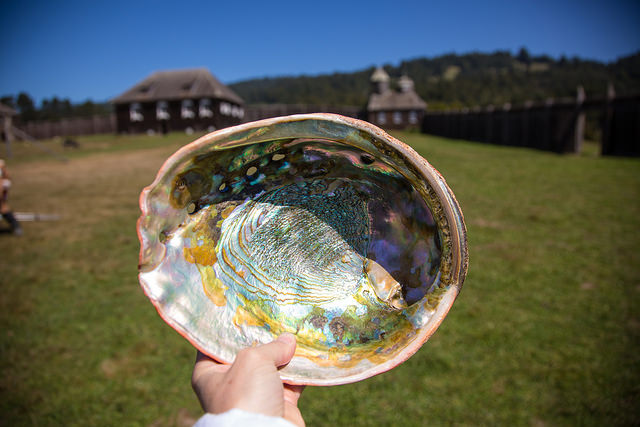
\includegraphics[scale=0.5]{abalone_shell.jpg}
	\caption{Abalone shell (by Nicki Dugan Pogue, CC BY-SA 2.0)}
\end{figure}
\subsection{开始}
这个导航用三个数据集,\href{http://download.tensorflow.org/data/abalone_train.csv}{abalone\_train.csv}包含训练数据3320样本。\href{http://download.tensorflow.org/data/abalone_test.csv}{abalone\_test.csv}包含标记测试数据850个样本。\href{http://download.tensorflow.org/data/abalone_predict.csv}{abalone\_predict}包含7个预测样本。
下面的章节一步步写Estimator代码,完整的代码在\href{https://www.github.com/tensorflow/tensorflow/blob/r1.4/tensorflow/examples/tutorials/estimators/abalone.py}{这里}
\subsection{载入abalone csv数据到TensorFlow数据集}
为了输入数据进model,你讲需要下载cvs文件载入到TensorFlow Dataset。首先添加一些标准的Python和TensorFlow导入,设置FLAGS:
\begin{lstlisting}[language=Python]
from __future__ import absolute_import
from __future__ import division
from __future__ import print_function

import argparse
import sys
import tempfile

# Import urllib
from six.moves import urllib

import numpy as np
import tensorflow as tf

FLAGS = None
\end{lstlisting}
开启采集\lstinline[language=Python]{tf.logging.set_verbosity(tf.logging.INFO)}

然后定义一个函数载入CSV文件:
\begin{lstlisting}[language=Python]
def maybe_download(train_data, test_data, predict_data):
  ""Maybe downloads training data and returns train and test file names.""
  if train_data:
    train_file_name = train_data
  else:
    train_file = tempfile.NamedTemporaryFile(delete=False)
    urllib.request.urlretrieve(
        "http://download.tensorflow.org/data/abalone_train.csv",
        train_file.name)
    train_file_name = train_file.name
    train_file.close()
    print("Training data is downloaded to %s" % train_file_name)

  if test_data:
    test_file_name = test_data
  else:
    test_file = tempfile.NamedTemporaryFile(delete=False)
    urllib.request.urlretrieve(
        "http://download.tensorflow.org/data/abalone_test.csv", test_file.name)
    test_file_name = test_file.name
    test_file.close()
    print("Test data is downloaded to %s" % test_file_name)

  if predict_data:
    predict_file_name = predict_data
  else:
    predict_file = tempfile.NamedTemporaryFile(delete=False)
    urllib.request.urlretrieve(
        "http://download.tensorflow.org/data/abalone_predict.csv",
        predict_file.name)
    predict_file_name = predict_file.name
    predict_file.close()
    print("Prediction data is downloaded to %s" % predict_file_name)

  return train_file_name, test_file_name, predict_file_name"
\end{lstlisting}
最后创建main()载入csv文件进入Datasets,定义flags允许用户通过命令行选择制定CSV文件训练,测试和预测数据集

\begin{lstlisting}[language=Python]
def main(unused_argv):
  # Load datasets
  abalone_train, abalone_test, abalone_predict = maybe_download(
    FLAGS.train_data, FLAGS.test_data, FLAGS.predict_data)

  # Training examples
  training_set = tf.contrib.learn.datasets.base.load_csv_without_header(
      filename=abalone_train, target_dtype=np.int, features_dtype=np.float64)

  # Test examples
  test_set = tf.contrib.learn.datasets.base.load_csv_without_header(
      filename=abalone_test, target_dtype=np.int, features_dtype=np.float64)

  # Set of 7 examples for which to predict abalone ages
  prediction_set = tf.contrib.learn.datasets.base.load_csv_without_header(
      filename=abalone_predict, target_dtype=np.int, features_dtype=np.float64)

if __name__ == "__main__":
  parser = argparse.ArgumentParser()
  parser.register("type", "bool", lambda v: v.lower() == "true")
  parser.add_argument(
      "--train_data", type=str, default="", help="Path to the training data.")
  parser.add_argument(
      "--test_data", type=str, default="", help="Path to the test data.")
  parser.add_argument(
      "--predict_data",
      type=str,
      default="",
      help="Path to the prediction data.")
  FLAGS, unparsed = parser.parse_known_args()
  tf.app.run(main=main, argv=[sys.argv[0]] + unparsed)
\end{lstlisting}
\subsection{实例化一个Estimator}
当使用一个tf.estimator提供的类定义一个模型(想DNNClassifier)的时候,你在结构体中应用正确的配置参数。
\begin{lstlisting}[language=Python]
my_nn = tf.estimator.DNNClassifier(feature_columns=[age, height, weight],
                                   hidden_units=[10, 10, 10],
                                   activation_fn=tf.nn.relu,
                                   dropout=0.2,
                                   n_classes=3,
                                   optimizer="Adam")
\end{lstlisting}
你不需要写任何代码说明TensorFlow如何训练模型,计算损失,返回预测;这些逻辑已经写入的DNNClassifier。

通过对比,当你创建你自己的estimator的时候,构造体接受两个高级参数用于模型的配置,model\_fn和parms:
\lstinline[language=Python]{nn = tf.estimator.Estimator(model_fn=model_fn, params=model_params)}
\begin{itemize}
\item model\_fn:一个包含所有的上面提到的逻辑的函数对象支持训练,估计和预测。你只管实现功能,下一章节\href{https://www.tensorflow.org/extend/estimators#constructing-modelfn}{ Constructing the model\_fn}构造包含创建一个模型函数的细节。
\item params:一个可选的词典超参数(学习率,dropout)等将被传输进model\_fn。
\end{itemize}
\begin{quote}
\textbf{注意:}\emph{像tf.estimator的预先定义的回归和分类器一样,Estimator初始化器也接受通常的配置参数model\_dir和config}
\end{quote}
对于abalone预测器,模型将接受一个超参数:学习率。在你的代码的开头定义LEARNING\_RATE作为,之后配置采集:
\begin{lstlisting}[language=Python]
tf.logging.set_verbosity(tf.logging.INFO)

# Learning rate for the model
LEARNING_RATE = 0.001
\end{lstlisting}
\begin{quote}
\textbf{注意:}\emph{这里的LEARING\_RATE设置为0.001,但是当你需要更好的结果时你可以在训练过程中改变这个值}
\end{quote}
然后,添加下面代码到main(),创建字典model\_params包含学习率和实例化的Estimator:
\begin{lstlisting}[language=Python]
# Set model params
model_params = {"learning_rate": LEARNING_RATE}

# Instantiate Estimator
nn = tf.estimator.Estimator(model_fn=model_fn, params=model_params)
\end{lstlisting}
\subsection{构造model\_fn}
Estimator API的基本的框架像这样:
\begin{lstlisting}[language=Python]
def model_fn(features, labels, mode, params):
   # Logic to do the following:
   # 1. Configure the model via TensorFlow operations
   # 2. Define the loss function for training/evaluation
   # 3. Define the training operation/optimizer
   # 4. Generate predictions
   # 5. Return predictions/loss/train_op/eval_metric_ops in EstimatorSpec object
   return EstimatorSpec(mode, predictions, loss, train_op, eval_metric_ops)
\end{lstlisting}
model\_fn必须接受三个参数:
\begin{itemize}
	\item features:一个包含通过input\_fn传递待模型的包含特征的字典
	\item labels:一个Tensor包含通过input\_fn传递到模型的标签。当model自己推理的时候将出现空的调用
	\item mode:一个\href{https://www.tensorflow.org/api_docs/python/tf/estimator/ModeKeys}{tf.estimator.ModeKeys}字符串值指明model\_fn被调用的上下文:
		\begin{itemize}
	\item tf.estimator.ModeKeys.TRAIN model\_fn调用在训练模式下,也就是通过train()调用
	\item tf.estimator.ModeKeys.EVAL model\_fn在估计模式下调用,也就是通过evaluate调用
	\item tf.estimator.ModeKeys.PREDICT model\_fn在预测模式下调用,也就是通过predict()调用
		\end{itemize}
\end{itemize}
model\_fn也接受一个包含用于训练的超参数参数(正如上面框架介绍的)

函数执行的主题跟着下面的任务(更多的细节查看下面的章节)
\begin{itemize}
		\item 配置模型,对于abalone预测器,浙江是一个神经网络
		\item 定义用于计算预测结果和目标值接近程度的损失函数。
		\item 定义一个训练操作制定优化算法最小化损失值的计算
\end{itemize}
model\_fn必须返回一个\href{https://www.tensorflow.org/api_docs/python/tf/estimator/EstimatorSpecC}{tf.estimator.EstimatorSpec}对象,包含下面的值:
\begin{itemize}
	\item mode(要求)。模型运行的模式,通常你将返回model\_fn的mode参数
	\item predictions(要求在PREDICT模式下)。一个字典映射你的选择的名字为包含模型预测的Tensor。例如\begin{lstlisting}[language=Python]{python predictions = {"results": tensor_of_predictions}},
在PREDICT模式,你在EstimatorSpec返回的字典将通过predict()返回,因此你可以用你想使用的方式构造它
	\item loss(要求EVAL和TRAIN模式)。一个包含有损失标量值的Tensor:模型损失函数(更深的讨论在\href{https://www.tensorflow.org/extend/estimators#defining_loss}{ Defining loss for the model})在输入计算后的的输出。这用于TRAIN模式用于处理错误和采集,自动作为度量包含在EVAL模式。
	\item train\_op:(仅仅要求在TRAIN模式)。一个返回训练步数的操作
	\item eval\_metric\_ops(可选)。一个name/value对制定当模型在EVAL模式下运行时制定将被计算的度量。你的选择的标签的名字用于度量,和你的度量计算的结果。\href{https://www.tensorflow.org/api_docs/python/tf/metrics}{tf.metrics}模块提供预定义的函数用于多种常规测量。
		下面的eval\_netric\_ops包含一个用tf.metrics.accuracy计算的accuracy方法:\begin{lstlisting}[language=Bash]{
			python eval_metric_ops = { "accuracy": tf.metrics.accuracy(labels, predictions) }}
		\end{lstlisting}
\end{itemize}
如果你没有指定evalue\_metric\_ops,仅仅loss将在估计的时候被计算。
\subsection{结合tf.feature\_column和tf.layers配置神经网络}
构造一个\href{https://en.wikipedia.org/wiki/Artificial_neural_network}{神经网络}需要创建和连接输入层,隐藏层和输出层。

输入层是一系列的节点(在模型中的一个特征),节点通过在features参数接受特征输入传入model\_fn。如果features包含一个包含你的特征数据的n维Tensor,然后他可能为输入层服务。如果features包含一个\href{https://www.tensorflow.org/tutorials/linear#feature_columns_and_transformations}{feature columns }通过输入函数人传递给模型,你可以结合\href{https://www.tensorflow.org/api_docs/python/tf/feature_column/input_layer}{tf.feature\_column.input\_layer}函数转化输入层Tensor。
\begin{lstlisting}[language=Python]
input_layer = tf.feature_column.input_layer(
    features=features, feature_columns=[age, height, weight])
\end{lstlisting}
正如上面显示的,input\_layer()接受两个参数:
\begin{itemize}
		\item features:一个从字符串到包含对应feature数据的Tensor映射,它在model\_fn中的features参数被明确的传递
		\item feature\_columns:一个模型中所有的FeatureColumns的列表(年龄,高度,重量(上面例子))
\end{itemize}
神经网络的输入层必须通过一个\href{https://en.wikipedia.org/wiki/Activation_function}{activation function}连接到一个或者更多的隐藏层对前面层的数据执行非线性变换。最后的隐藏层然后连接最后一层的输出层。tf.layers提供tf.layers.dense函数构造全连接层。激活函数通过activation参数控制,一些选项传递给activation参数:
\begin{itemize}
	\item tf.nn.relu 下面的代码通过\href{https://en.wikipedia.org/wiki/Rectifier_(neural_networks)}{ReLU activation function}(\href{https://www.tensorflow.org/api_docs/python/tf/nn/relu}{tf.nn.relu})创建一个全连接到前一层input\_layer的层
	\item tf.nn.relu 后面的代码通过ReLU6激活函数创建一个和hidden\_layer的全连接层全连接单元层(\href{https://www.tensorflow.org/api_docs/python/tf/nn/relu6}{tf.nn.relu})
	\item None下面的代码没有激活函数创建一个和前一层second\_hidden\_layer全连接的单元层,仅仅是一个线性变换
		\begin{lstlisting}[language=Bash]
		python output_layer = tf.layers.dense( inputs=second_hidden_layer, units=3, activation=None)
		\end{lstlisting}
\end{itemize}
其他可能的激活函数,例如
\begin{lstlisting}[language=Python]
output_layer = tf.layers.dense(inputs=second_hidden_layer,
                               units=10,
                               activation_fn=tf.sigmoid)
\end{lstlisting}
上面的代码创建一个用sigmoid激活函数(\href{https://www.tensorflow.org/api_docs/python/tf/sigmoid}{tf,sigmoid})和second\_hidden\_layer全连接的output\_layer,更多预定义函数的细节查看\href{https://www.tensorflow.org/api_guides/python/nn#activation_functions}{API docs}
将它们放在一起,下面的代码构造一个完整的神经网络用于Abalone预测器和捕获他的预测:
\begin{lstlisting}[language=Python]
def model_fn(features, labels, mode, params):
  """Model function for Estimator."""

  # Connect the first hidden layer to input layer
  # (features["x"]) with relu activation
  first_hidden_layer = tf.layers.dense(features["x"], 10, activation=tf.nn.relu)

  # Connect the second hidden layer to first hidden layer with relu
  second_hidden_layer = tf.layers.dense(
      first_hidden_layer, 10, activation=tf.nn.relu)

  # Connect the output layer to second hidden layer (no activation fn)
  output_layer = tf.layers.dense(second_hidden_layer, 1)

  # Reshape output layer to 1-dim Tensor to return predictions
  predictions = tf.reshape(output_layer, [-1])
  predictions_dict = {"ages": predictions}
  ...
\end{lstlisting}
这里因为你将用numpy\_input\_fn传递abalone的Datasets,features是一个字典{'X':data\_tensor},因此features["x"]是输入层,网络包含两个隐藏层,每个层有10个结合ReLU激活函数的节点。输出层没有激活函数\href{https://www.tensorflow.org/api_docs/python/tf/reshape}{tf.reshape}一个一维tensor捕获模型的预测存储在predicions\_dict。
\subsection{为模型定义一个损失}
model\_fn返回的EstimatorSpec必须包含loss:一个代表loss值的Tensor,用来衡量模型在训练和评估运行时预测反映的结果的好坏。\href{https://www.tensorflow.org/api_docs/python/tf/losses}{tf.losses}模块提供方便的函数用多种度量计算损失,包括:
\begin{itemize}
	\item absolute\_difference(labels,predictions)使用\href{https://en.wikipedia.org/wiki/Deviation_(statistics)#Unsigned_or_absolute_deviation}{absolute-difference formula}(正如$L_1$损失)计算损失
\item log\_loss(labels,predictions)用\href{https://en.wikipedia.org/wiki/Loss_functions_for_classification#Logistic_loss}{logistic loss forumula }计算损失函数(通常使用逻辑回归)
\item mean\_squared\_error(labels,predictions)使用\href{https://en.wikipedia.org/wiki/Mean_squared_error}{mean squared error}计算损失($L_2$损失)
\end{itemize}
下面的例子使用mean\_squared\_error()添加一个定义的loss到abalone的model\_fn
\begin{lstlisting}[language=Python]
def model_fn(features, labels, mode, params):
  """Model function for Estimator."""

  # Connect the first hidden layer to input layer
  # (features["x"]) with relu activation
  first_hidden_layer = tf.layers.dense(features["x"], 10, activation=tf.nn.relu)

  # Connect the second hidden layer to first hidden layer with relu
  second_hidden_layer = tf.layers.dense(
      first_hidden_layer, 10, activation=tf.nn.relu)

  # Connect the output layer to second hidden layer (no activation fn)
  output_layer = tf.layers.dense(second_hidden_layer, 1)

  # Reshape output layer to 1-dim Tensor to return predictions
  predictions = tf.reshape(output_layer, [-1])
  predictions_dict = {"ages": predictions}

  # Calculate loss using mean squared error
  loss = tf.losses.mean_squared_error(labels, predictions)
  ...
\end{lstlisting}
查看\href{https://www.tensorflow.org/api_guides/python/contrib.losses}{API guide}了解更多loss函数的使用和支持的参数。

丰富的估计度量可以被添加到一个eval\_metric\_ops字典。下面的代码定义一个rmse度量,计算模型预测的均方误误差。注意labels tensor转化一个float64类型为predictions匹配的类型的tensor,包含真的值:
\begin{lstlisting}[language=Python]
eval_metric_ops = {
    "rmse": tf.metrics.root_mean_squared_error(
        tf.cast(labels, tf.float64), predictions)
}
\end{lstlisting}
\subsection{定义为model训练操作}
训练操作定义优化算法TensorFlow将你拟合模型到训练数据上是使用。通常当训练的时候,目标是最小化误差。一个简单的方法创建训练操作是实例化一个tf.train.Optimizer子类和调用minimize方法。
下面的代码为abalone的model\_fn定义一个训练操作使用损失值计算\href{https://www.tensorflow.org/extend/estimators#defining_loss}{ Defining Loss for the Model},学习率传递到params中的函数,梯度下降优化器。对于global\_step,方便的函数\href{https://www.tensorflow.org/api_docs/python/tf/train/get_global_step}{tf.train.get\_global\_step}考虑生成一个整数变量。
\begin{lstlisting}[language=Python]
optimizer = tf.train.GradientDescentOptimizer(
    learning_rate=params["learning_rate"])
train_op = optimizer.minimize(
    loss=loss, global_step=tf.train.get_global_step())
\end{lstlisting}
对于优化器的完整列表查看\href{https://www.tensorflow.org/api_guides/python/train#optimizers}{API guid}
\subsection{完整的abalone model\_fn}
这里最终,完整的model\_fn用于abalone年龄预测器。下面的代码配置神经网络,定义损失和训练操作;返回一个EstimatorSpec对象包含mode,predictions\_dict,loss和train\_op:
\begin{lstlisting}[language=Python]
def model_fn(features, labels, mode, params):
  ""Model function for Estimator.""

  # Connect the first hidden layer to input layer
  # (features["x"]) with relu activation
  first_hidden_layer = tf.layers.dense(features["x"], 10, activation=tf.nn.relu)

  # Connect the second hidden layer to first hidden layer with relu
  second_hidden_layer = tf.layers.dense(
      first_hidden_layer, 10, activation=tf.nn.relu)

  # Connect the output layer to second hidden layer (no activation fn)
  output_layer = tf.layers.dense(second_hidden_layer, 1)

  # Reshape output layer to 1-dim Tensor to return predictions
  predictions = tf.reshape(output_layer, [-1])

  # Provide an estimator spec for `ModeKeys.PREDICT`.
  if mode == tf.estimator.ModeKeys.PREDICT:
    return tf.estimator.EstimatorSpec(
        mode=mode,
        predictions={"ages": predictions})

  # Calculate loss using mean squared error
  loss = tf.losses.mean_squared_error(labels, predictions)

  # Calculate root mean squared error as additional eval metric
  eval_metric_ops = {
      "rmse": tf.metrics.root_mean_squared_error(
          tf.cast(labels, tf.float64), predictions)
  }

  optimizer = tf.train.GradientDescentOptimizer(
      learning_rate=params["learning_rate"])
  train_op = optimizer.minimize(
      loss=loss, global_step=tf.train.get_global_step())

  # Provide an estimator spec for `ModeKeys.EVAL` and `ModeKeys.TRAIN` modes.
  return tf.estimator.EstimatorSpec(
      mode=mode,
      loss=loss,
      train_op=train_op,
      eval_metric_ops=eval_metric_ops)"
\end{lstlisting}
\subsection{运行Abalone模型}
你已经为abalone年龄预测器初始化一个Estimator在model\_fn中定义它的行为;所有需要做的是训练,估计,和预测。
字啊面的代码是main()的结尾,拟合神经网络训练数据和估算精度。
\begin{lstlisting}[language=Python]
train_input_fn = tf.estimator.inputs.numpy_input_fn(
    x={"x": np.array(training_set.data)},
    y=np.array(training_set.target),
    num_epochs=None,
    shuffle=True)

# Train
nn.train(input_fn=train_input_fn, steps=5000)

# Score accuracy
test_input_fn = tf.estimator.inputs.numpy_input_fn(
    x={"x": np.array(test_set.data)},
    y=np.array(test_set.target),
    num_epochs=1,
    shuffle=False)

ev = nn.evaluate(input_fn=test_input_fn)
print("Loss: %s" % ev["loss"])
print("Root Mean Squared Error: %s" % ev["rmse"])))
\end{lstlisting}
\begin{quote}
\textbf{注意:}\emph{上面的代码用输入若函数输入features(x)和label(y) Tensor到模型中训练(train\_input\_fn)和估计test\_input\_fn,了解更多输入函数,查看}\href{https://www.tensorflow.org/get_started/input_fn}{Building Input Functions with tf.EstimatorSpec}
\end{quote}
然后运行代码,你应该看到类似下面的输出:
\begin{lstlisting}[language=Python]
...
INFO:tensorflow:loss = 4.86658, step = 4701
INFO:tensorflow:loss = 4.86191, step = 4801
INFO:tensorflow:loss = 4.85788, step = 4901
...
INFO:tensorflow:Saving evaluation summary for 5000 step: loss = 5.581
Loss: 5.581
\end{lstlisting}
损失得分被报告是当运行ABALONE\_TEST数据集来自model\_fn的军方误差。
为ABALONE\_PREDICT数据集预测年龄,添加下面代码到main():
\begin{lstlisting}[language=Python]
# Print out predictions
predict_input_fn = tf.estimator.inputs.numpy_input_fn(
    x={"x": prediction_set.data},
    num_epochs=1,
    shuffle=False)
predictions = nn.predict(input_fn=predict_input_fn)
for i, p in enumerate(predictions):
  print("Prediction %s: %s" % (i + 1, p["ages"]))))
\end{lstlisting}
这里predict()函数迭代的返回结果在predictions。for训练返回结果,返回代码类似下面:
\begin{lstlisting}[language=Bash]
...
Prediction 1: 4.92229
Prediction 2: 10.3225
Prediction 3: 7.384
Prediction 4: 10.6264
Prediction 5: 11.0862
Prediction 6: 9.39239
Prediction 7: 11.1289
\end{lstlisting}
\subsection{附加资源}
祝贺你,你已经从Estimator成功地构建了一个tf.estimator。更多关于构建Estimator的资料查看下面的API章节:
\begin{itemize}
\item \href{https://www.tensorflow.org/api_guides/python/contrib.layers}{Layers}
\item \href{https://www.tensorflow.org/api_guides/python/contrib.losses}{Losses}
\item \href{https://www.tensorflow.org/api_guides/python/contrib.layers#optimization}{Optimization}
\end{itemize}
\section{TensorFlow用其他语言}
\subsection{背景}
这个文档是针对那些想要在其他语言中创造或者开发TensorFlow功能的开发者。它描述了TensorFlow的特性和在其它编程语言中使用的推荐步骤。

Python是TensorFlow支持的首选语言,当前支持的特性最多。更多的函数正在被移植进TensorFlow(C++实现)核心通过\href{https://www.github.com/tensorflow/tensorflow/blob/r1.4/tensorflow/c/c_api.h}{C API},客户端语言应该用语言的\href{https://en.wikipedia.org/wiki/Foreign_function_interface}{外部函数接口}调用这个\href{https://www.github.com/tensorflow/tensorflow/blob/r1.4/tensorflow/c/c_api.h}{C API}提供TensorFlow函数。
\subsection{概览}
在其它编程语言中提供TensorFlow功能可能分为下面多种情况:
\begin{itemize}
\item 运行一个预先定义好的图:给一个GraphDef(或者MetaGraphDef)protocol消息,能创建一个绘画,运行查询得到tensor结果。对于想上手机app或者服务器来说通过预先训练好的模型推理足够的
\item 图接口:每定义一个TensorFlow操作至少定义一个函数或者添加一个操作到图上。理想的这些函数将被自动生成因此他们保持同步直到操作的定义被修改
\item 梯度(AKA自动微分):给一个图和输入输出操作列表,添加操作到图上计算输出与对应输入的偏微分(梯度)。对于图上的类似操作允许定义梯度函数
\item 函数:定义一个在GraphDef中能被多处调用的子图。在FunctionDefLibrary定义一个FunctionDef包含在GraphDef
\item 控制流:如果用户指定子图,构造if和while。最好的情况是他们和梯度一起工作
\item 神经网络库:一些组件结合在一起支持创建神经网络模型和训练他们(可能是分布式设置)。在其它语言有这些将很方便,当前没有计划支持Python外的其他语言。这些库同上面这些特性的包装器
\end{itemize}
在一个小的,语言绑定应该支持运行一个预先定义的图,但是多数应该支持图的构建。TensorFlow Python API提供所有的这些特性。
\subsection{当前状态}
新的语言支持应该建立的\href{https://www.github.com/tensorflow/tensorflow/blob/r1.4/tensorflow/c/c_api.h}{C API}之上。然而,正如下表所见,不是所有的函数在C中都可用。为\href{https://www.github.com/tensorflow/tensorflow/blob/r1.4/tensorflow/c/c_api.h}{C API}提供更多支持的计划正在进行
\begin{table}[!h]
	\begin{tabular}{|p{4cm}|p{6cm}|p{4.7cm}|}
\hline
特性&Python&C\\
\hline
运行一个预定义的图&tf.import\_graph\_def, tf.Session&	TF\_GraphImportGraphDef, TF\_NewSession\\
\hline
结合生成的操作构造图&Yes	&Yes (The C API supports client languages that do this)\\
\hline
梯度&tf.gradients	&\\
\hline
函数&tf.python.framework.function.Defun&\\
\hline
控制流&tf.cond, tf.while\_loop&\\	
\hline
神经网络库&tf.train, tf.nn, tf.contrib.layers, tf.contrib.slim&\\
\hline
\end{tabular}
	\caption{语言支持}
	\label{tab:ex7_1}
\end{table}
\newline
\textbf{推荐方法}\newline
\subsection{运行一个预定义的图}
语言绑定希望定义下面的类:
\begin{itemize}
\item Graph:一个图表示一个TensorFlow计算。有一些对应C API的TF\_Graph的操作组成,主要用作创建操作和启动会话的参数。在图(TF\_GraphNextOperation)上也支持迭代,通过名字(TF\_GraphOperationByName)查看操作转换为或者从GraphDef rotocol消息(TF\_GraphToGraphDef和TF\_GraphImportGraphDef)转换
\item Operation:表示图上的一个计算节点。对应C API中的TF\_Operation
\item Output:表示图中操作的输出。有一个DataType(和最终的形状)也许作为输入参数传送给一个函数进行加操作,或者对于一个Session的Run()方法获取tensor作为输出。对应C API的TF\_Output。
\item Session:表示TensorFlow运行环境的类似实例的一个客户端呢。主要工作是构造一个Graph和在图上调用Run()选项。对应C API中的一个TF\_Session。
\item Tensor表示数据类型为DataType的N维数组。获取数据进出Session的Run()调用。对应C API的TF\_Tensor。
\item DataType:一些TensorFlow支持的可能的类型,对应C API中的TF\_DataType和Python API中的dtype对应
\end{itemize}
\subsection{图的构造}
TensorFlow有一些操作和列表不是静态的,因此我们推荐通过手写生成添加操作到图上(军官厚些一些是一个好的找出生成器应该生成什么),需要生成一个包含一个OpDef protocol消息的函数。有一些方法获取注册操作的OpDefs列表:
\begin{itemize}
\item 在CAPI中的TF\_GetAllOpList获取所有祖册的OpDef protocol消息。这可能用用于客户端语言写生成器。这要求客户端语言为了解释OpDef消息有Protocol buffer支持
\item  C++函数OpRegistry::Global()->GetRegisteredOps()返回所有注册的OpDef的相同的列表(定义在tensorflow/core/framework/op.h)。这可以用与在C++(对于没有protocol buffer 支持的语言来说特别管用)
写生成器
\item 通过一个自动的处理ASCII序列版本被周期性的检查tensorflow/core/ops/ops.pbtxt
\begin{itemize}
\item 在CameICase中操作的名字。为了按照语言习惯生成函数。例如,如果语言使用snake\_case,使用CameICase态体操作的函数名称
\item 一个输入和输出列表。对于一字儿通过属性访问的多台,如在\href{https://www.tensorflow.org/extend/adding_an_op}{Adding an op}描述
\item 一些属性值是否认的。注意一些将被自动推断(如果他们由输入决定),一些将可选(如果他们有一个默认),一些将要要求(非默认),
\item 常用操作,输入,输出和非推理的属性的文档
\item 一些通过运行环境使用的领域可能被代码生成器胡萝卜
\end{itemize}
\end{itemize}
一个OpDef能转化为text函数添加用TF\_OperationDescription C API添加操作到图上(打包语言的外部函数接口)
\begin{itemize}
\item 开始TF\_NewOperation()创建TF\_OperationDescription*
\item 当输入(依赖于是否输入有一个列表类型)调用TF\_AddInput()或者TF\_AddInputList()
\item Call TF\_SetAttr*()函数设置非推理的属性。如果你不想覆盖默认值也许跳过属性
\item 如果需要设置选项范围
\begin{itemize}
\item TF\_SetDevice():抢播操作到指定设备
\item TF\_AddControlInput():添加请求在一个操作开始前另一个操作完成前
\item TF\_SetAttrString("\_kernel")设置内核标记(很少使用)
\item TF\_ColocateWith()布置一个操作
\end{itemize}
\item 调用TF\_FinishOperation()调用时,添加这个操作到图上,之后不能被修改
\end{itemize}
存在样本运行代码代码生成器作为构建程序(Bazel genrule)的一部分。带把生成能用一个自动的cron程序运行,可能在结果中检测。这在生成代码和OpDef的生成之间创建一个分歧进入仓库。但是对于go语言的go get和Rust cargoops希望代码之前生成期望被生成的情况。在最后,对于一些语言代码可能从tensorflow/core/ops/ops.pbtxt动态生成。
\subsection{处理常数}
如果用户可以提佛那个仓鼠给输入参数调用将边的更简单。生成的代码转化常熟为操作添加到图上用于作为输入对操作被实例化。
\subsection{可选参数}
如果语言允许对一个函数(想关键字参数(默认使用Python))的可选参数,为可选属性,操作名称,设备,控制输入等使用阿门。在一些语言中这些选项参数可以用于动态scopes(像Python的with块)。没有这些特性,库也许如在C++版本的而TensorFlow API存储构建的样本。
\subsection{Name scopes}
用一些scope问津结构支持命名图的操作是一个好的想法,特别是考虑TensorBoard依赖它用合理的方式显示大图。Python和C++有不同的方法:在Python中,使用with块,目录作为名字的一部分。有一个本地线程栈结合scopes定义名字层级结构。名称的最新组件通过用户明确使用或者按照操作被默认添加。在C++中名字的目录部分存储在Scopes对象。NewSubScope()方法添加名字的一部分返回一个新的Scope。最新的名字的组件用WithOpName()方法设置,想Python默认的通过添加的操作命名。Scope对象明确的传递指定的名字。
\subsection{包装器}
确保一些函数的私有属性以至于包装器函数做一点额外的工作可能就被替代。这也给一个escape 从生成代码的scope外支持特性。

包装器的一个用法是支持SparseTensor输入输出,一个SparseTensor是一个三个dense tensor的SparseTensor:索引,值,和形状。值是响亮的大小n,形状是响亮的rank,索引时一个矩阵[n,rank]。

另一个原因四用包装器保持状态。有一些这样的操作(例如变量)有一些同伴操作用于操作状态。在Python API有类用于操作,操作的构造体创建op,类的方法添加组件到图上操作状态。
\subsection{其它的考虑}
\begin{itemize}
		\item 它有些关键字用于和语言关键字(或者其他符号哦将残生困难,想库函数的名字或者生成的代码中的变量引用)冲突的关键字重命名操作函数和参数
		\item 通常对于添加一个Const操作到图上的函数是一个包装器因此生成的函数将有同于的DataType输入
\end{itemize}
\subsection{梯度,函数和控制流}
在这里支持梯度,函数和控制流操作在Python外的语言中不可用,当\href{https://www.github.com/tensorflow/tensorflow/blob/r1.4/tensorflow/c/c_api.h}{C API}提供需要的支持后这将被跟新。
\section{一个TensorFlow模型文见得开发者工具}
大多数用户不需要考虑TensorFlow存储在磁盘中文件的内部细节,但是如果你是一个工具开发者也许需要考虑。
例如你也许想分析模型或者在TensorFlow和其他格式之间转化。这个向导尝试向你解释一些你如何结合主要文件保存模型数据
的详细工作,确保容易开发一些工具。
\subsection{Protocol Buffers}
所有的TensorFlow的文件格式都是基于\href{https://developers.google.com/protocol-buffers/?hl=en}{Protocol Buffers}
,因此熟悉它是如何工作的很有价值。总结来说你在文本文件中定义数据结构,protobuf用C,Python或者你可以载入的其他语言生成
类,以一种友好的方式访问数据。我们经常认为Protocol Buffers作为protobufs,我们将在这个向导中使用用这个
这个惯例。
\subsection{GraphDef}
在TensorFlow中图对象是计算的基础。这包含一些节点组成的网络,每个节点代表一个操作,节点作为输入或者输出
被连接到其它节点,你可以通过调用as\_default\_def()保存它,返回一个GraphDef对象。

GraphDef类是一个定义在
\href{https://github.com/tensorflow/tensorflow/blob/master/tensorflow/core/framework/graph.proto}{tensorflow/core/framework/graph.proto}定义的ProtoBuf库创建的GraphDef类。
protobuf工具解析这个文本文件,生成代码载入,存储和操作图定义。如果你看到一个标准的TensorFlow
文件表示一个模型,它很可能包含protobuf代码保存的一些列序列化的的GraphDef对象。这个生成代码
用于保存和从文件中载入GraphDef文件。代码通常像下面这样载入这个模型
\lstinline[language=Python]{graph_def = graph_pb2.GraphDef()}
这行创建一个空的GraphDef对象,这个类从定义在grapg.proto中定义的本质文件创建。这个对象将从我们的文件
操作这个对象
\lstinline[language=Python]{with open(FLAGS.graph,"rb") as f}
这里我们传递进脚本一个路径获取文件
\begin{lstlisting}[language=Python]
if FLAGS.input_binary:
  graph_def.ParseFromString(f.read())
else:
  text_format.Merge(f.read(), graph_def)
\end{lstlisting}
\subsubsection{文本或者二进制}
事实上一个Protobuf我们可以存储进入两种不同的格式。文本格式是一个人类可读的形式,对于调试和编辑
十分方面,但是当有一些想权重的数值数据存储文本格式的文件将很大。你可以查看\href{https://github.com/tensorflow/tensorboard/blob/master/tensorboard/demo/data/graph_run_run2.pbtxt}{graph\_run\_run2.pbtxt}一个晓得样本
二进制文件相比文本文件小得多,尽管他们对我们不可读,在这个脚本,我们要求用户应用一个flag指示
师傅输入是二进制还是文本,因此我们知道正确的函数调用。你可以在\href{https://storage.googleapis.com/download.tensorflow.org/models/inception_v3_2016_08_28_frozen.pb.tar.gz}{inception\_v3 archive}
找到一个大型二进制文件样本。正如inception\_v3\_2016\_08\_28\_frozen.pb。
这个API本身可以有一些让人困惑,二进制调用事实上是ParseFromString(),然而我们用一个来自text\_format模块的使用函数
载入原始的文件。
\subsection{Nodes}
当你载入一个文件进入graph\_def变量时,你可以访问里面的数据,对于多数常见目的,重要的章节是节点列表
存储在节点数目中。这里的代码循换处理这个操作
\lstinline[language=Python]{for node in graph_def.node}
每个节点是一个NodeDef对象,定义在\href{https://github.com/tensorflow/tensorflow/blob/master/tensorflow/core/framework/node_def.proto}{tensorflow/core/framework/node\_def.proto}
,这是TensorFlow图的基本构建模块,每个定义的单独操作用输入连接,这里的number是NodeDef。
\subsubsection{name}
每个节点应该有一个独一无二的id,不被其他的图中的节点使用。如果你不指定一个作为你用Python API构建一个graph。
一个翻译到操作的名字上,想"MatMul"和单调递增的数连接,像为你选择"5",名字被用于定义两个节点的连接。
当运行时为你的整个图设置输入和输出。
\subsubsection{op}
这定义了运行的操作,例如"Add","MatMul"或者"Conv2"。当一个图运行的时候,op的名字被在实现中注册查找。
注册通过调用REGISTER\_OP()宏操作。像在
\href{https://github.com/tensorflow/tensorflow/blob/master/tensorflow/core/ops/nn\_ops.cc}{tensorflow/core/ops/nn\_ops.cc}
\subsubsection{input}
一个字符串列表,列表中每个元素是其他节点的名字,通常跟着引号和输出端口。例如,一个节点和两个输入有一个像
["some\_node\_name","another\_node\_name"],等价于["some\_node\_name:0","another\_node\_name:0"]
定义节点的第一个输入作为节点的来自“some\_node\_name”的第一个输出,第二个输入来自"anather\_node\_name"的
第一个输出。
\subsubsection{device}
在大多数情况下你可以忽略这个,因为它定义在分布式环境下节点运行的位置,或者什么时候你想强制操作运行在
CPU或者GPU上。
\subsubsection{attr}
这是一个key/value存储节点的的属性。有节不变的参数,一些在像卷积滤波器的尺寸不改变。或者常数操作
的值。因为有如此多不同类型的属性值,对于字符串,对证书或者tensor值的数组,这里有一个分割的protobuf
文件定义的数据结构保存他们,在
\href{https://github.com/tensorflow/tensorflow/blob/master/tensorflow/core/framework/attr_value.proto}{tensorflow/core/framework/attr\_value.proto.}
每个属性有一个独一无二的名字字符串,期待的属性被列出然后操作被定义。如果一个属性被节点呈现。
但是如果一个操作定义中的默认的列表,默认被用于图的创建。你可以通过调用node.name访问所有的数据,node.op等
在Python中节点列表列表存储在GraphDef是一个模型架构的完整定义。
\subsection{Freezing}
一个让人难以理解的是训练中的权重不被存储在文件中。相反,他们被保存在
单个的checkpoint文件中,在graph中的Variable操作,当他们被初始化的时候
载入最新的值,因此有\href{https://github.com/tensorflow/tensorflow/blob/master/tensorflow/python/tools/freeze_graph.py}{freeze\_graph.py }
脚本接受一个图定义和一些checkpoint文件同时freeze他们到一个单独的文件,载入GraphDef的时候,
从最新的chepoint文件获取所有变量的值,当取代Variable操作和Const权重的数值数据存储在他的属性中,
然后剔除额外的不能用于钱箱推理的节点,vaocun输出结果的GraphDef进一个输出文件。
\subsection{权重格式}
如果你正在处理TensorFlow模型表达的神经网络模型,一个常见的问题是提取和解释权重值。一个通用的
方法存储他们,例如在图中freezed\_graph脚本创建,它作为Const操作包含作为Tensors的权重。这些定义在
\href{https://github.com/tensorflow/tensorflow/blob/master/tensorflow/core/framework/tensor.proto}{tensorflow/core/framework/tensor.proto}
包含数据的类型和尺寸,正如值本身。在Python中,你通过NodeDef从一个NodeDef操作获取TensorProto对象表达一个Const操作
通过调用想some\_node\_def.attr['value'].tensor。

这样给你一个权重数据的对象表达。数据将被存储在有suffix\_val的列表中作为对象类型的索引,例如float\_val对于32位浮点数据类型。
卷及权重的顺序经常对于处理在不同的框架中转化有技巧的。在TensorFlow中,滤波器权重对于Conv2D操作被存储在第二行。
期待的数据顺序[filter\_height,filter\_width,input\_depth,output\_depth],这里filter\_count随着
内存中一个邻接的值滑动平均增加。
